\section{Instala\c{c}\~ao para Windows}
\begin{flushleft}
O download do COQ \'{e} encontrado no endere\c{c}o: \begin{center}\textbf{http://coq.inria.fr/download.}\\
\end{center}
\begin{figure}[!htb]
\centering
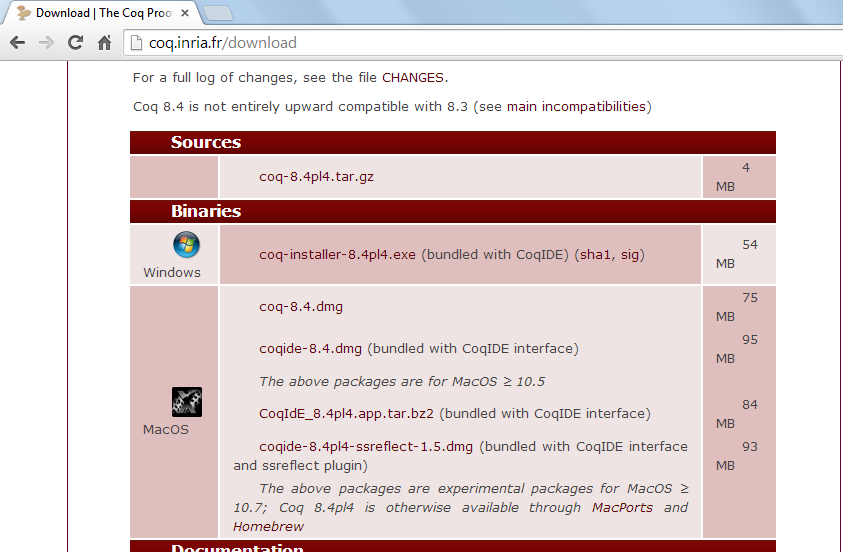
\includegraphics[scale=0.4]{1.png}
\end{figure}
Para continuar a instala\c{c}\~{a}o seguir os passos indicados:\\
Para Prosseguir com a instala\c{c}\~{a}o clique next como indicado:
\begin{figure}[!htb]
\centering
\includegraphics[scale=0.4]{w3.png} 
\end{figure}
Reveja os termos da licen\c{c}a antes de instalar, se voc\^{e} aceita-los clique em I agree.Para instalar voc\^{e} deve aceitar os termos de uso.
\begin{figure}[!htb]
\centering
\includegraphics[scale=0.4]{w4.png}
\end{figure}
Verifique os componentes que voc\^{e} deseja instalar e desmarque os componentes que n\~{a}o deseja instalar. Clique em Next para continuar.
\begin{figure}[!htb]
\centering
\includegraphics[scale=0.4]{w5.png}
\end{figure}
Escolha a pasta na qual deseja instalar o Coq e em seguida clique em Install para iniciar a instala\{c}\~{a}o.
\begin{figure}[!htb]
\centering
\includegraphics[scale=0.4]{w6.png} 
\end{figure}
Aguarde enquanto o Coq \'{e} instalado, para mais detalhes clique em show details.
\begin{figure}[!htb]
\includegraphics[scale=0.4]{w7.png}
\end{figure}  
Coq foi instalado no seu computador, clique em Finish para fechar este assistente.
\begin{figure}[!htb]
\centering
\includegraphics[scale=0.4]{w8.png} 
\end{figure}
\end{flushleft} 
